\newpage
\subsection{Учет отходов производства (макулатуры)}

 

Вся макулатура в виде отходов производства передается в пресс. Прессовщик взвешивает получившийся после пресса тюк макулатуры. Тюк вывозится для хранения в специально отведенное место.  
Каждую смену прессовщики передают мастеру бланки с указанием количества произведенных тюков макулатуры (рис. \ref{pic:III.3}). Мастер в системе 1С: УПП формирует акт.
Бухгалтер на основании акта ставит макулатуру на приход в системе 1С: УПП. Макулатура перерабатывается на ООО ''ПЗБМ''.



\textbf{Учет брака}

Брак, выявленный на складе, возвращается в производство на основании акта, составленного ОУК. 

Отгрузка готовой продукции со склада выполняется по факту (за вычетом брака).
%Зависшие остатки и брак кладовщик списывает в системе СБИС документом “Списание со склада”. 
%После списания брака кладовщик составляет и передает в ОТК  отчет  для расчета брака %(рис. \ref{pic:d31}).



% Мастер смены смотрит по наполнению, заказывают фуру и отгружает по мягкой накладной. Могут отвозить на другую площадку газелью и оттуда уже отгружать на продажу.
% Вся макулатура с обеих цехов привозится на пресс.
% В макулатурном прессу ведется журнал учета макулатуры (рис. \ref{pic:photo19}). На тюки крепится ярлык с весом и числом. При отгрузке макулатуры на склад выписывается форма (рис.  \ref{pic:pic_a33_1}), т.ж. каждый день подаются сведения в Отдел ГОГП (рис.  \ref{pic:pic_a34}).


% %  êîíöå ñìåíû ïðåñîâùèê ôîðìèðóåò îò÷åò (ñì. ôîðìó ''Îò÷åò ïî çàïðåñîâàííîé ìàêóëàòóðå çà ñìåíó'' \ref{pic:WasteReport2}). Îò÷åò ïåðåäàåòñÿ ìàñòåðó ïðîèçâîäñòâà.


\clearpage
\begin{figure}
\begin{center}
 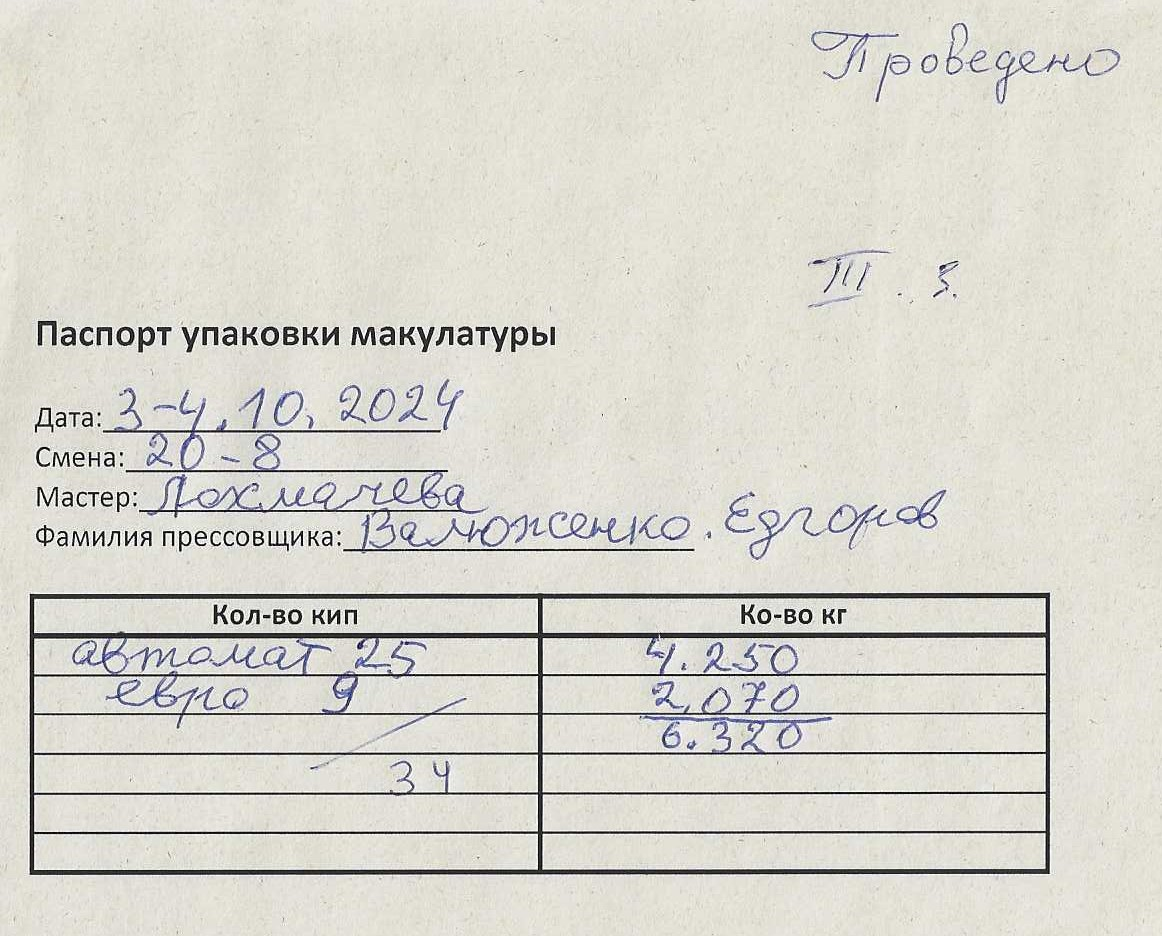
\includegraphics[height=0.5\textheight, keepaspectratio]{Pics/III.3.jpg}
\end{center}
 \caption{Паспорт упаковки макулатуры}
 \label{pic:III.3}
\end{figure}
% \begin{figure}
% \begin{center}
%   \includegraphics[height=0.6\textheight, keepaspectratio]{Pics/pic_a33_1.jpg}
% \end{center}
%   \caption{Рапорт по отгрузке макулатуры}
%   \label{pic:pic_a33_1}
% \end{figure}
%\clearpage

% \begin{figure}
% \begin{center}
%   \includegraphics[height=0.6\textheight, keepaspectratio]{Pics/pic_a34.jpg}
% \end{center}
%   \caption{Рапорт машиниста по макулатуре}
%   \label{pic:pic_a34}
% \end{figure}
% \clearpage


\clearpage
\ifx \notincludehead\undefined
\normalsize
\end{document}
\fi